\documentclass[compress,xcolor={dvipsnames}]{beamer}
\usepackage{fancyvrb,newverbs} % For customized verbatim
\usepackage{calligra} % A fancy text for ending `Thank you'
\usepackage[T1]{fontenc}
\usepackage{outline}
\usepackage{changepage}
\usefonttheme[onlymath]{serif}

\author{Zihang Wang}
\title{Phase Field Tutorial}
\subtitle{Phase Field Simulation of Spinodal Decomposition}
\institute{Central South University}

\AtBeginSubsection[]
{
	\begin{frame}
		\tableofcontents[sectionstyle=show/shaded,subsectionstyle=show/shaded/hide,subsubsectionstyle=show/shaded/hide]
	\end{frame}
}
\usetheme{Berlin}

\setbeamertemplate{footline} {
    \begin{beamercolorbox}[ht=2.5ex,dp=1.125ex,
      leftskip=.3cm,rightskip=.3cm plus1fil]{title in head/foot}
      {\usebeamerfont{institute in head/foot}\usebeamercolor[fg]{institute in head/foot}\insertshortinstitute}
      \hfill
      {\centering\usebeamerfont{title in head/foot}\insertshortsubtitle}
      \hfill
      {\usebeamerfont{frame number}\usebeamercolor[fg]{frame number}\insertframenumber~/~\inserttotalframenumber}
    \end{beamercolorbox}
    \begin{beamercolorbox}[colsep=1.5pt]{lower separation line foot}
    \end{beamercolorbox}
}

% ---------------------------------------------------------------------------
\definecolor{cverbbg}{gray}{0.93}

\newenvironment{cverbatim}
 {\SaveVerbatim{cverb}}
 {\endSaveVerbatim
  \flushleft\fboxrule=0pt\fboxsep=.5em
  \colorbox{cverbbg}{\BUseVerbatim{cverb}}%
  \endflushleft
}
\newenvironment{lcverbatim}
 {\SaveVerbatim{cverb}}
 {\endSaveVerbatim
  \flushleft\fboxrule=0pt\fboxsep=.5em
  \colorbox{cverbbg}{%
    \makebox[\dimexpr\linewidth-2\fboxsep][l]{\BUseVerbatim{cverb}}%
  }
  \endflushleft
}
\newverbcommand{\cverb}
  {\setbox\verbbox\hbox\bgroup}
  {\egroup\colorbox{cverbbg}{\box\verbbox}}

\setlength{\parindent}{2em}

\newcommand{\bhref}[2]{
    \href{#1}{\color{blue}{#2}}
}
% ---------------------------------------------------------------------------

\begin{document}
\begin{frame}
    \titlepage
    \begin{figure}[!h]
        \centering
        
\includegraphics[width=0.18\linewidth]{pic/csulogo.jpg}
        
\includegraphics[width=0.25\linewidth]{pic/MInDes_Icon.jpg}
    \end{figure}
\end{frame}

\begin{frame}
    \tableofcontents[currentsection, hideothersubsections, sectionstyle=show/show]
\end{frame}

% ---------------------------------------------------------------------------
\section{Review \& Intro}
\begin{frame}
    \frametitle{Quick Review}
    Finally, we shall start our phase field simulation now. But before that, What have we got in the last tutorial?

    \begin{itemize}
        \item C++ Introduction
        \item C++ Environment Setup
        \item Basic C++ Usage
        \item Algorithm Implementation with C++
        \item Simple Simulation Example
    \end{itemize}

    Now, we shall have a look at today's simulation example: spinodal decomposition.

\end{frame}

\subsection{Spinodal Decomposition}
\begin{frame}
    \frametitle{What is Spinodal Decomposition}

    Spinodal decomposition is one of the solid state phase transformation, usually a phase separation in alloy solid solution. Below is an image of spinodal decomposition simulation result, which we will obtain at the end of this tutorial.

    \begin{figure}
        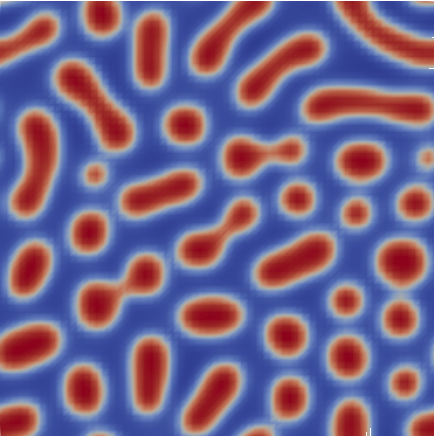
\includegraphics[width=0.4\linewidth]{pic/spinodal_image.png}
    \end{figure}

\end{frame}

\begin{frame}
    \frametitle{Phase Diagram and Free Energy Curve}

    As a phase transformation, let's have a look at its phase diagram:\vspace{-5pt}
    \begin{columns}
        \begin{column}{.5\linewidth}
            \begin{figure}
                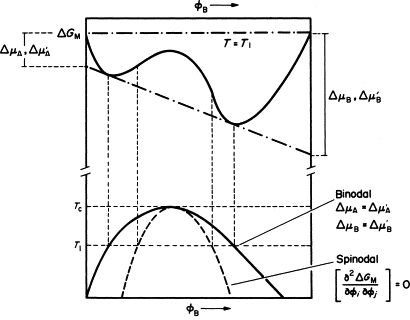
\includegraphics[width=1.\linewidth]{pic/energy_pd.jpg}
            \end{figure}
        \end{column}
        \begin{column}{.5\linewidth}
            The lower part of this graph is phase diagram, and the upper part is the free energy profile under temperature \emph{T1}. Dash line in phase diagram stands for \emph{spinodal line}, corresponding to points \(\frac{\partial ^2 G}{\partial \phi ^2} = 0\). And, \(\frac{\partial ^2 G}{\partial \phi ^2} < 0\) inside the dash line, which is instable region for this system.
        \end{column}
    \end{columns}
    \vspace{5pt}
    When the concentration inside the miscibility gap is fluctuated a little, the concentration will separate to the valleys of free energy curve, and hence spinodal decomposition.

\end{frame}

\begin{frame}
    \frametitle{Spinodal Decomposition, Cahn--Hilliard \& Phase Field}

    Let's talk a little about history. Spinodal decomposition is firstly reported inside Cu-Ni-Fe alloy in the early 1940s, and then some explanation were given. Based on Ginzburg--Landau free energy model, John W. Cahn and John Hilliard developed a free energy model that can be decribed as a function of concentration \(c\) and concentration gradient, \(\nabla c\), which is:
    \[
        F = \int_\omega f_b + \kappa \left( \nabla c \right)^2 \,\mathrm{d}\Omega.
    \]
    And to evolute the decomposition process, a generalized diffusion equation, which is also known as `Cahn--Hilliard' equation, is used:
    \[
        \frac{\partial c}{\partial t} = M \nabla^2 \mu.
    \]
    This shall be the originate of phase field simulation method.

\end{frame}

\subsection{Today's Target}
\begin{frame}
    \frametitle{A-B Alloy's Spinodal Decomposition}

    Instead of investigating a real problem related to spinodal decomposition using phase field method, we are going to investigate a imaginary alloy with two simple composition: A and B, and this alloy, under certain temperature, has an extremly simple free energy curve such that we can easily describe it using the following polynomial:
    \[
        f(c) = Ac^2(1-c)^2,
    \]
    which is also known as \emph{double well potential}.  The free energy curve of this function when \(A = 1\) can be plot as:

\end{frame}

\begin{frame}
    \frametitle{A-B Alloy's Spinodal Decomposition}
    \begin{figure}
        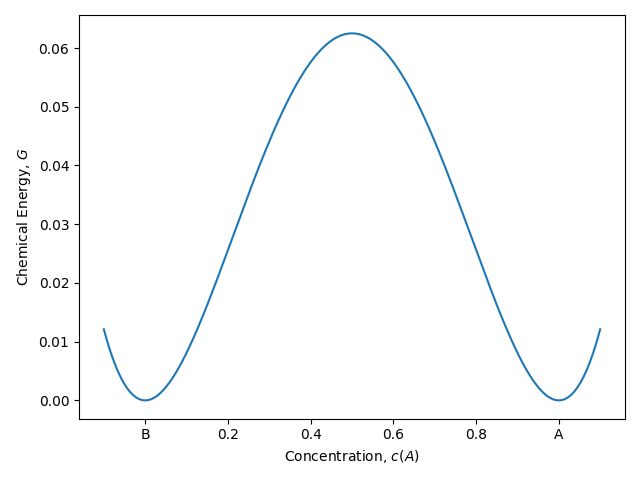
\includegraphics[width=0.5\linewidth]{pic/AB_free_energy.png}
    \end{figure}
    \vspace{-5pt}
    As you can see, this free energy curve indicates that, the alloy with concentration at the middle of the curve will eventually decompose and separate into two phase, with one phase full of element A (\(c = 1.0\)), and another phase full of element B (\(c = 0.0\)).

\end{frame}

\begin{frame}
    \frametitle{What shall we do?}

    Here is our goal for today's tutorial:
    \begin{itemize}
        \item Analyse the question and prepare for the simulation
        \item Write C++ program to simulate AB alloy spinodal decomposition
        \item Analyse the simulation result
    \end{itemize}

    So in brief, just complete this simulation. Let's do it now.

\end{frame}

\section{Simulation}
\subsection{Preparation}
\begin{frame}[fragile]
    \frametitle{Parameter List}
    \begin{center}
        \vspace{-20pt}
        \begin{adjustwidth}{-10pt}{}
            \begin{tabular}{ccc}
                \hline
                Parameters                         & Value                       & Type           \\
                \hline
                \(N_x\) \& \(N_y\)                 & 64                          & \cverb|int|    \\
                \(\mathrm{d}x\) \& \(\mathrm{d}y\) & 1.0                         & \cverb|double| \\
                \(\mathrm{d}t\)                    & 0.01                        & \cverb|double| \\
                simulation step (\cverb|nstep|)    & 10000                       & \cverb|int|    \\
                output step (\cverb|pstep|)        & 50                          & \cverb|int|    \\
                initial concentration (\cverb|c0|) & 0.4                         & \cverb|double| \\
                concentration noise (\cverb|dc|)   & 0.1                         & \cverb|double| \\
                noise type                         & average random distribution & -              \\
                mobility \(M\) (\cverb|mobility|)  & 1.0                         & \cverb|double| \\
                gradient coefficient \(\kappa\)    & 0.5                         & \cverb|double| \\
                free energy parameter \(A\)        & 1.0                         & \cverb|double| \\
                boundary condition                 & periodic                    & -              \\
                boundary value truncate            & 1e-6                        & \cverb|double| \\
                \hline
            \end{tabular}
        \end{adjustwidth}
    \end{center}

\end{frame}

\begin{frame}
    \frametitle{Formulae to Use}
    Time iterate:
    \[
        \scriptstyle
        c^{n+1}_{i,j} = c^n_{i,j}+ \Delta t  M \nabla^2 \left( \frac{\delta F_{ij}}{\delta c} \right)^n;
    \]
    Energy variation:
    \[
        \scriptstyle
        \left( \frac{\delta F_{ij}}{\delta c} \right)^n = \mu\left(c^n_{ij}\right) - \kappa\nabla^2c^n_{ij};
    \]
    Chemical potential:
    \[
        \scriptstyle
        \mu(c^n_{i,j}) = 2A(c^n_{i,j}(1-c^n_{i,j})^2 - ((c^n_{i,j})^2 (1-c^n_{i,j})));
    \]
    Total free energy:
    \begin{align*}
        \scriptstyle
        F &
        \scriptstyle
        = \sum_i^{Nx}\sum_{j}^{Ny}f(c_{i,j}) \\
          &
        \scriptstyle
        + \frac{\kappa}{2}\left( \sum_i^{Nx-1}\sum_{j}^{Ny-1}(c_{i+1,j}-c_{i,j})^2 + \sum_i^{Nx-1}\sum_{j}^{Ny-1}(c_{i,j+1}-c_{i,j})^2 \right) .
    \end{align*}
\end{frame}

\begin{frame}[fragile]
    \frametitle{Code Structure}

    Here the code structure to accomplish the simulation is presented as follows:
    \begin{columns}
        \begin{column}{.5\linewidth}
            \begin{itemize}
                \item Headers
                \item Tool Functions
                      \begin{itemize}
                          \item Free energy derivative
                          \item Laplacian calculation
                          \item Data output
                      \end{itemize}
                \item Constants
            \end{itemize}
        \end{column}
        \hspace{-20pt}
        \begin{column}{.5\linewidth}
            \begin{itemize}
                \item \cverb|main| function
                      \begin{itemize}
                          \item Mesh initialization
                          \item Time step loop
                          \item Mesh loop
                          \item Boundary check
                          \item Calculation
                          \item Time iterate
                          \item Data output
                      \end{itemize}
            \end{itemize}
        \end{column}
    \end{columns}

\end{frame}

\subsection{Code Implementation}
\begin{frame}
    \frametitle{Write It Now}

    Now let's write this simulation by hand from scratch.

    The completed code will be avaliable after this tutorial.

\end{frame}
\subsection{Results}
\begin{frame}
    \frametitle{Visualization}

    We choose Paraview to open the data files we generated from the program, which are mainly the \emph{vtk} files, and some energy curves.

\end{frame}

\section{Summary}
\begin{frame}
    \frametitle{Summary}

    This should be the first example of phase field simulation. By writing this code by hand, the simulation step, especially the calculation process should be clear.

    Spinodal decomposition is a good start point of phase field simulation, where you can try various solving method about it, for example, finite element method, Fourier spectum method and so on. It's simple enough and matches the phase field method well.

    However, there are still a lot we can do about this simulation. For example, try to couple the concentration field with other physical fields, such as mechanical field, temperature field and so on. That's beyond this tutorial's scope, but we will see an example about two field exist and evolute together in the next tutorial.

\end{frame}

\begin{frame}
    \frametitle{Exercise}

    Below are some exercises for today's contents:

    \begin{enumerate}
        \item Please try to write today's code and run it by yourself.
        \item Modify the parameters related to the free energy and governing equation, for example, the gradient coefficient \(\kappa\) and analyse the results.
        \item Modify the parameters related to the calculation, for example, \(\mathrm{d}x\) or \(\mathrm{d}t\), and analyse the results. Please be careful when adjust them as these parameters might influence the stability of the calculation.
    \end{enumerate}

    Besides these exercises, you are encouraged to try modifying the simulation model by yourself to see the influence.

\end{frame}

\begin{frame}
    \frametitle{Resources}

    Here are some resources that might help you.
    \begin{itemize}
        \item Today's contents are mainly from the book we have been always refered to, \emph{Programming Phase Field Modeling}. You will find matlab\textsuperscript{\textregistered} code in this book about today's simulation. You are welcomed to translate the matlab\textsuperscript{\textregistered} code into C++ or other programming language.
        \item For the result visualization, \emph{vtk} file format is used. For more information about this file format, you can refer to \bhref{https://docs.vtk.org/en/latest/design_documents/VTKFileFormats.html}{VTK file format reference}.
    \end{itemize}
\end{frame}

\begin{frame}
    \begin{center}
        {\Huge \calligra Thanks!}
        \bigbreak
        {\huge Any questions are welcomed!}
    \end{center}
\end{frame}

\end{document}

